%% ============================================================
%%  Série Avaliação na Prática — FGV CLEAR
%%  Guia de Uso de Evidências Acadêmicas no Ciclo da Política Pública
%% ============================================================

% !TEX program = pdflatex
% !TEX encoding = UTF-8 Unicode

\documentclass[12pt, a4paper, openany]{book}

%% ── Codificação e Idioma ────────────────────────────────────
\usepackage[utf8]{inputenc}
\usepackage[T1]{fontenc}
\usepackage[brazil]{babel}

%% ── Fonte ───────────────────────────────────────────────────
\usepackage{tgpagella}

%% ── Matemática ──────────────────────────────────────────────
\usepackage{amsmath, amssymb, amsfonts, dsfont, amsthm}

%% ── Figuras e Tabelas ───────────────────────────────────────
\usepackage{graphicx, float}
\usepackage[labelfont=bf, font=small, justification=justified]{caption}
\usepackage{subcaption}
\usepackage{booktabs, multirow, multicol, array}
\usepackage{longtable}
\usepackage{tabularx}

%% ── Layout ──────────────────────────────────────────────────
\usepackage{geometry}
\geometry{a4paper, left=2.5cm, right=2.5cm, top=2.5cm, bottom=2.5cm}
\usepackage{setspace}
\onehalfspacing
\usepackage{fancyhdr}
\usepackage{emptypage}
\usepackage{enumitem}
\usepackage{parskip}
\usepackage{microtype}
\usepackage{url}

%% ── Cores (paleta CLEAR) ────────────────────────────────────
\usepackage{xcolor}
\definecolor{clearblue}{HTML}{1B3A6E}
\definecolor{clearlightblue}{HTML}{5CA4A9}
\definecolor{cleardarkblue}{HTML}{003F72}
\definecolor{cleargray}{HTML}{6E6E6E}
\definecolor{salmonbg}{RGB}{252,235,230}
\definecolor{salmonframe}{RGB}{230,160,140}
\definecolor{bluebg}{RGB}{235,245,251}
\definecolor{blueframe}{RGB}{58,125,181}
\definecolor{orangebg}{RGB}{254,245,231}
\definecolor{orangeframe}{RGB}{230,126,34}
\definecolor{redbg}{RGB}{250,230,225}
\definecolor{redframe}{RGB}{180,40,40}
\definecolor{codebg}{RGB}{248,248,248}
\definecolor{codeframe}{RGB}{200,200,200}

%% ── Hyperlinks e Bibliografia ───────────────────────────────
\usepackage{hyperref}
\hypersetup{
  colorlinks=true,
  linkcolor=clearlightblue,
  citecolor=clearlightblue,
  urlcolor=clearlightblue,
  pdfauthor={FGV CLEAR},
  pdftitle={Guia de Uso de Evidências Acadêmicas no Ciclo da Política Pública}
}
\usepackage[round, authoryear]{natbib}

%% ── TColorbox ───────────────────────────────────────────────
\usepackage[many]{tcolorbox}
\tcbuselibrary{breakable, skins}

%% ── Código ──────────────────────────────────────────────────
\usepackage{listings}

%% ── Cabeçalhos e Rodapés ────────────────────────────────────
\pagestyle{fancy}
\fancyhf{}
\fancyhead[R]{\small\color{clearblue}\textit{Guia CLEAR $|$ Uso de Evid\^encias Acad\^emicas}}
\fancyfoot[C]{\thepage}
\renewcommand{\headrulewidth}{0.4pt}
\renewcommand{\headrule}{\hbox to\headwidth{\color{clearblue}\leaders\hrule height \headrulewidth\hfill}}

%% ── Títulos de Seção ────────────────────────────────────────
\usepackage{titlesec}
\titleformat{\chapter}[display]
  {\normalfont\huge\bfseries\color{clearblue}}
  {\chaptertitlename\ \thechapter}{20pt}{\Huge}
\titleformat{\section}
  {\normalfont\Large\bfseries\color{clearblue}}{\thesection}{1em}{}
\titleformat{\subsection}
  {\normalfont\large\bfseries\color{cleardarkblue}}{\thesubsection}{1em}{}
\titleformat{\subsubsection}
  {\normalfont\normalsize\bfseries\color{cleardarkblue}}{\thesubsubsection}{1em}{}

%% ── Caixas Temáticas ────────────────────────────────────────
\newtcolorbox{destaquebox}[1][Destaque]{
  enhanced, breakable,
  colback=salmonbg, colframe=salmonframe, coltitle=black, fonttitle=\bfseries,
  title=#1, boxrule=0.5pt, arc=2pt,
  left=6pt, right=6pt, top=4pt, bottom=4pt
}
\newtcolorbox{notabox}[1][Nota]{
  enhanced, breakable,
  colback=bluebg, colframe=blueframe, coltitle=white, fonttitle=\bfseries,
  title=#1, boxrule=0.5pt, arc=2pt,
  left=6pt, right=6pt, top=4pt, bottom=4pt
}
\newtcolorbox{conexaobox}[1][Conex\~ao com a s\'erie]{
  enhanced, breakable,
  colback=orangebg, colframe=orangeframe, coltitle=black, fonttitle=\bfseries,
  title=#1, boxrule=0.5pt, arc=2pt,
  left=6pt, right=6pt, top=4pt, bottom=4pt
}
\newtcolorbox{exemplobox}[1][Exemplo]{
  enhanced, breakable,
  colback=salmonbg, colframe=salmonframe, coltitle=black, fonttitle=\bfseries,
  title=#1, boxrule=0.5pt, arc=2pt,
  left=6pt, right=6pt, top=4pt, bottom=4pt
}
\newtcolorbox{atencaobox}[1][Aten\c{c}\~ao]{
  enhanced, breakable,
  colback=redbg, colframe=redframe, coltitle=white, fonttitle=\bfseries,
  title=#1, boxrule=0.5pt, arc=2pt,
  left=6pt, right=6pt, top=4pt, bottom=4pt
}

%% ── Metadados de Figuras/Quadros ────────────────────────────
\newcommand{\figmeta}[3]{%
  \par\vspace{4pt}%
  \begin{minipage}{\linewidth}%
  \footnotesize%
  \textbf{Fonte:} #1%
  \ifx&#2&\else\\\textbf{Elabora\c{c}\~ao:} #2\fi%
  \ifx&#3&\else\\\textbf{Nota:} #3\fi%
  \end{minipage}%
  \vspace{6pt}%
}

%% ── Profundidade de numera\c{c}\~ao ─────────────────────────
\setcounter{secnumdepth}{2}
\setcounter{tocdepth}{2}

\begin{document}
\frontmatter

% ─── CAPA ────────────────────────────────────────────────────────────────────
\thispagestyle{empty}
\begin{center}
\vspace*{3cm}

{\Large\bfseries\color{clearlightblue} SÉRIE: AVALIAÇÃO NA PRÁTICA}

\vspace{1.5cm}

{\Huge\bfseries\color{clearblue}
  Guia de Uso de\\[0.3cm]
  Evidências Acadêmicas\\[0.3cm]
  no Ciclo da\\[0.3cm]
  Política Pública}

\vspace{2cm}

{\large FGV CLEAR $|$ FGV EESP}

\vspace{0.5cm}
{\large Maio de 2026}

\vfill

\vspace{0.5cm}
\noindent\textcolor{clearlightblue}{\rule{\textwidth}{0.6pt}}
\vspace{0.3cm}

\begin{minipage}{0.92\textwidth}
\centering
\vspace*{10em}
{\small\textbf{Resumo}}\\[0.4em]
\small\setlength{\parindent}{0pt}
Este guia foi desenvolvido para gestores públicos e consultores que
desejam incorporar evidências acadêmicas ao seu trabalho de forma prática e
crítica. Organizado a partir do Ciclo da Política Pública na abordagem do FGV
CLEAR \citep{Lima2025}, o guia percorre as cinco etapas do ciclo ---
identificação do problema, formulação, implementação, análise de resultados e
tomada de decisão --- mostrando como a pesquisa científica pode ser mobilizada
em cada uma delas. Os primeiros capítulos apresentam os principais tipos de
publicações acadêmicas e orientam sobre como encontrá-las de forma eficiente,
com atenção a fontes de prestígio e rigor metodológico. Os capítulos seguintes
ilustram, com exemplos aplicados, como as evidências contribuem para
diagnósticos mais precisos, políticas mais bem fundamentadas, implementações
mais robustas e avaliações mais críveis. O guia se encerra com uma discussão
sobre os limites e as armadilhas do uso acrítico da literatura acadêmica.
\end{minipage}

\vspace{0.3cm}
\noindent\textcolor{clearlightblue}{\rule{\textwidth}{0.6pt}}
\end{center}
\newpage

% ─── FICHA TÉCNICA ───────────────────────────────────────────────────────────
\thispagestyle{empty}
\section*{Ficha Técnica}

\textbf{Equipe técnica:} Alei Fernandes Santos, André Portela Souza, Caio de Souza Castro, Carol Imura, Gustavo Nebó Garcia, Júlia Brant Araújo Pereira da Silva, Lycia Lima, Michel Szklo.

\vspace{1cm}

\noindent\textbf{Apresentação.} Este guia integra a série de publicações
\textit{Avaliação na Prática}, desenvolvida pelo FGV CLEAR com o objetivo de
ampliar o acesso a conhecimentos sobre monitoramento e avaliação com foco em
políticas públicas.

Fundado em 2015, o FGV CLEAR tem se dedicado ao fortalecimento da cultura de
gestão orientada por evidências no Brasil e em países lusófonos. Com sede na
Escola de Economia de São Paulo da Fundação Getulio Vargas (FGV EESP), o FGV
CLEAR atua como centro regional da Iniciativa CLEAR (\textit{Centers for
Learning on Evaluation and Results}).

Saiba mais sobre o FGV CLEAR e acesse outras publicações em:
\textbf{www.fgvclear.org}

\newpage

% ─── SOBRE ESTE GUIA ─────────────────────────────────────────────────────────
\thispagestyle{empty}
\section*{Sobre este guia}
Quem gere uma política pública não precisa começar do zero a cada
decisão. Existe um acervo considerável de pesquisa acadêmica sobre quase
tudo o que se queira saber. Efeitos de transferências de renda
condicionadas a comportamento. Retornos da educação para anos adicionais
de estudo em diferentes níveis. Eficácia comparada de diferentes desenhos
de programas de saúde pública. Impactos de intervenções em segurança
pública testadas em dezenas de cidades. O problema, na maioria das vezes,
não é a ausência de evidência. É o conjunto de passos entre a evidência
que existe e a decisão que precisa ser tomada.

Cada um desses passos tem suas armadilhas. Localizar evidência hoje vai
além de ``buscar no Google Scholar''. Existem bases especializadas
(Campbell Collaboration, J-PAL, 3ie, Cochrane na saúde) que consolidam
pesquisa de qualidade em formato apropriado para quem decide e não para
quem produz, com revisões sistemáticas e mapas de evidência que poupam
tempo de quem não pode passar semanas lendo papers individuais. Saber que
essas bases existem e quando usá-las já é meio caminho.

Julgar a qualidade da evidência é o passo seguinte, e exige distinguir
um estudo bem desenhado de um mal desenhado mesmo sem formação
metodológica completa. Algumas heurísticas práticas levam longe sem virar
técnica especializada. Existe um grupo de comparação no estudo? Como ele
foi formado? O estudo foi pré-registrado antes da coleta de dados, ou os
resultados foram analisados várias vezes até produzir o que apareceu
publicado? O efeito reportado foi consistente em outras amostras ou só
apareceu naquela? Perguntas como essas, feitas com método, separam
evidência convincente de evidência fraca.

Decidir sobre aplicabilidade é o passo onde mais coisa dá errado. Um
programa que funcionou em Massachusetts pode não funcionar em Pernambuco.
Não por motivo místico, mas porque o programa interage com o contexto
que o recebe: estrutura institucional, qualidade da implementação,
características da população, presença de outros programas que reforçam
ou conflitam. Validade externa é a propriedade de uma estimativa que
permite (ou não) sua aplicação a outro contexto, e julgar isso é parte do
trabalho do gestor que vai usar o resultado. Significa pensar sobre quais
condições do estudo original são essenciais para o efeito ter aparecido,
e quais condições estão presentes ou ausentes no contexto onde a política
seria replicada.

Traduzir, finalmente, é integrar a evidência ao ciclo da política
pública. Diagnóstico do problema (a evidência ajuda a identificar quais
aspectos do problema são mais tratáveis e quais não). Formulação (a
evidência sugere quais desenhos funcionaram em contextos parecidos).
Implementação (a evidência aponta os mecanismos pelos quais o programa
produz efeito e portanto onde o cuidado de implementação importa mais).
Avaliação (a evidência prévia orienta o desenho da avaliação local,
incluindo as hipóteses a testar). Em cada etapa, a evidência acadêmica
entra como insumo, não como veredicto.

Este guia foi escrito para esse percurso. É para gestores e técnicos que
trabalham com decisões reais, não com a produção de novas pesquisas. A
leitura não substitui formação metodológica, mas ajuda a fazer as
perguntas certas antes de contratar uma avaliação cara, antes de adotar
uma intervenção lida em relatório, e antes de descartar uma alternativa
por intuição quando há evidência sólida disponível.
\newpage

% ─── COMO LER ESTE GUIA ──────────────────────────────────────────────────────
\thispagestyle{empty}
\section*{Como ler este guia}
Três tipos de caixa estruturam a leitura, identificados por cor:
\vspace{0.3cm}
\begin{notabox}[Caixa azul --- pontos-chave]
Aparece ao fim de cada capítulo, com sínteses e recomendações para quem
precisa decidir.
\end{notabox}
\begin{exemplobox}[Caixa verde --- exemplo aplicado]
Mostra como as ideias do capítulo se traduzem em situações de política
pública. Os casos são fictícios, mas calibrados por padrões recorrentes
na literatura e na prática de gestão.
\end{exemplobox}
\begin{atencaobox}[Caixa vermelha --- cuidados essenciais]
Sinaliza armadilhas comuns --- pontos em que uma escolha mal fundamentada
compromete toda a análise.
\end{atencaobox}
\vspace{0.5cm}
\noindent O guia faz referência recorrente ao \textit{Guia CLEAR de
Monitoramento e Avaliação de Políticas Públicas: do diagnóstico à decisão}
\citep{Lima2025} --- doravante \textbf{Guia CLEAR de M\&A} ---, que trata
em profundidade as etapas do ciclo da política pública adotado na série.
Quando o texto menciona Teoria da Mudança, plano de monitoramento ou
tipologia de avaliações, é nesse guia que o leitor encontra o
desenvolvimento completo.
\newpage

% ─── SUMÁRIO ─────────────────────────────────────────────────────────────────
\tableofcontents

\mainmatter

% ═══════════════════════════════════════════════════════════════════════════════
% INTRODUÇÃO
% ═══════════════════════════════════════════════════════════════════════════════
\chapter*{Introdução}
\addcontentsline{toc}{chapter}{Introdução}
\markboth{Introdução}{}

A gestão pública avançou muito nas últimas décadas na incorporação de dados e
indicadores ao processo decisório. Sistemas de monitoramento, painéis de gestão
e registros administrativos tornaram-se ferramentas cada vez mais presentes no
cotidiano de gestores e consultores. No entanto, há uma fonte de conhecimento
que ainda é subutilizada nesse processo: a pesquisa acadêmica.

As razões para esse distanciamento são compreensíveis. Grande parte da produção
científica é escrita em linguagem altamente técnica, voltada para um público
especializado, o que pode tornar sua leitura árida e pouco acessível para quem
atua na gestão. O acesso também representa uma barreira concreta: muitos
periódicos científicos estão disponíveis apenas mediante assinatura
institucional, dificultando a consulta por equipes que não estão vinculadas a
universidades ou centros de pesquisa \citep{Oliver2014}. Somam-se a isso o
volume e a extensão dos artigos --- que raramente oferecem sínteses objetivas
orientadas para a decisão --- e a pressão do tempo, característica permanente
da gestão pública, que deixa pouco espaço para leituras longas e densas
\citep{Head2010}. O resultado é um distanciamento que empobrece a prática:
políticas formuladas sem diálogo com o conhecimento acumulado tendem a repetir
erros já documentados e a desperdiçar recursos em intervenções cujos limites já
são conhecidos.

Artigos científicos, revisões sistemáticas, meta-análises e \textit{policy
briefs} acumulam anos de investigação rigorosa sobre o que funciona --- e o que
não funciona --- em políticas públicas de diferentes áreas e contextos. Ignorar
esse repertório é abrir mão da possibilidade de aprender com o que outros já
fizeram, evitar erros conhecidos e fundamentar escolhas com base em evidências
testadas e com rigor metodológico \citep{Nutley2007}.

A pesquisa acadêmica, quando bem conduzida, oferece uma base sólida para
responder a perguntas que estão no centro da gestão pública: \textit{esse
problema realmente existe e qual sua magnitude? Essa intervenção já foi testada
em algum lugar? Quais foram os efeitos observados?} São perguntas que
acompanham todo o ciclo da política pública --- e este guia mostra como a
literatura acadêmica pode ajudar a respondê-las.

Este guia foi desenvolvido para gestores públicos e consultores que desejam
incorporar evidências acadêmicas ao seu trabalho de forma prática e crítica.
Ele está organizado a partir do Ciclo da Política Pública na abordagem do FGV
CLEAR \citep{Lima2025}, que estrutura o processo de formulação e gestão de
políticas em cinco etapas principais. A \textbf{identificação do problema} é o
ponto de partida: trata-se de compreender com precisão qual situação demanda
intervenção do Estado --- isoladamente ou mediante parcerias ---, suas causas,
sua magnitude e os grupos afetados. A \textbf{formulação} é o momento de
desenhar a intervenção --- definir objetivos, selecionar alternativas e
construir a lógica causal que conecta as ações aos resultados esperados. A
\textbf{implementação} diz respeito à execução da política na prática:
mobilização de recursos, entrega dos serviços e acompanhamento operacional. A
etapa de \textbf{resultados e impactos} busca compreender o que a política
efetivamente produziu --- para quem, em que magnitude e a que custo. Por fim,
a \textbf{tomada de decisão} é o momento em que as evidências acumuladas ao
longo do ciclo informam escolhas sobre a continuidade, expansão, reformulação
ou encerramento da política. A avaliação, nessa abordagem, não é uma etapa
isolada, mas uma prática transversal que deve estar presente ao longo de todo
o ciclo.

O guia acompanha esse percurso de ponta a ponta. Os dois primeiros capítulos
oferecem uma base conceitual e instrumental: o Capítulo~\ref{cap1} apresenta os
principais tipos de publicações acadêmicas e o que as torna fontes confiáveis
de conhecimento; o Capítulo~\ref{cap2} orienta como encontrá-las de forma
eficiente. Os quatro capítulos seguintes (Capítulos~\ref{cap3} a~\ref{cap6})
percorrem as etapas do ciclo da política pública --- diagnóstico, formulação,
implementação e análise de resultados --- mostrando como as evidências
acadêmicas podem ser utilizadas em cada etapa, com exemplos aplicados em
diferentes áreas de política pública. O guia se encerra com um capítulo
dedicado aos limites do uso de evidências.

Algumas ressalvas orientam a leitura. Evidências acadêmicas não substituem o conhecimento do contexto local, as informações advindas do monitoramento nem a capacidade institucional --- complementam e ajudam a qualificar. A ausência de evidências sobre uma intervenção não significa que ela não funciona; significa que ainda não foi suficientemente estudada. E nem toda publicação acadêmica tem a mesma qualidade --- parte do trabalho de usar bem a literatura é distinguir estudos robustos de achados frágeis ou enviesados \citep{Parkhurst2017}, tema retomado nos Capítulos~\ref{cap1} e~\ref{cap7}.

Este guia não pretende ser exaustivo. O objetivo é oferecer um ponto de entrada para que gestores e consultores incorporem o diálogo com a pesquisa acadêmica ao seu repertório de trabalho.

% ═══════════════════════════════════════════════════════════════════════════════
% CAPÍTULO 1
% ═══════════════════════════════════════════════════════════════════════════════
\chapter{O que são evidências acadêmicas e por que elas importam}\label{cap1}

Para muita gente, ``usar evidências'' em política pública evoca planilhas, relatórios técnicos ou dados administrativos. Mas há outro tipo de conhecimento que costuma ficar de fora: as evidências produzidas pela pesquisa acadêmica.

Este capítulo apresenta o que são essas evidências, quais são seus principais
formatos e o que as torna uma fonte valiosa --- e, ao mesmo tempo, exigente ---
para quem trabalha com políticas públicas.

\section{O que torna uma evidência ``acadêmica''?}

Uma evidência acadêmica é aquela produzida a partir de um processo sistemático
de investigação, orientado por métodos claros e cientificamente reconhecidos,
revisado por pares e publicado em canais reconhecidos pela comunidade
científica. Isso a distingue, por exemplo, de uma reportagem jornalística, de
um relatório institucional ou de uma percepção de gestor --- não porque essas
outras fontes sejam irrelevantes, mas porque o processo de produção acadêmica
oferece salvaguardas específicas contra vieses, erros de interpretação e
generalizações prematuras \citep{Gough2012}.

Na prática, o que mais interessa ao gestor público não é a origem da evidência,
mas o que ela revela com confiabilidade. A pesquisa acadêmica, quando bem
conduzida, oferece justamente isso: uma base mais sólida para responder a
perguntas como ``esse problema realmente existe e qual sua magnitude?'',
``essa intervenção já foi testada em algum lugar?'' ou ``quais foram os
efeitos observados?''.

\section{Tipos de publicações acadêmicas}

Não existe um único formato de publicação acadêmica. Para quem está começando a
navegar por esse universo, entender as diferenças entre os principais tipos
ajuda a escolher o material mais adequado a cada momento do ciclo da política
pública.

\subsection{Artigos científicos originais}

São o formato mais comum da produção acadêmica. Apresentam os resultados de uma
pesquisa específica --- seja um estudo de caso, uma análise estatística, uma
avaliação de impacto ou uma investigação qualitativa. São publicados em
periódicos científicos e passam por revisão por pares, ou seja, são avaliados
por outros pesquisadores especialistas na mesma área de estudo antes de serem
aceitos.

Para o gestor público, artigos científicos são especialmente úteis quando se
quer compreender os efeitos de uma intervenção específica em um contexto
determinado. A limitação é que um único artigo raramente é suficiente para
embasar uma decisão, uma vez que os resultados podem não se replicar em outros
contextos.

\subsection{Revisões sistemáticas}

Uma revisão sistemática reúne, de forma estruturada e transparente, todos os
estudos disponíveis sobre uma determinada pergunta de pesquisa. O objetivo é
sintetizar o estado do conhecimento sobre um tema, avaliando criticamente cada
estudo incluído e identificando padrões, inconsistências e lacunas na
literatura \citep{Higgins2019}.

Para quem toma decisões em políticas públicas, as revisões sistemáticas são
frequentemente o ponto de partida mais indicado. Elas oferecem uma visão
panorâmica do que já se sabe sobre uma intervenção, sem depender de um único
estudo.

\subsection{Meta-análises}

A meta-análise aprofunda a revisão sistemática: além de reunir os estudos
existentes, ela os combina estatisticamente para produzir uma estimativa
quantitativa do efeito médio de uma intervenção. Quando bem conduzida, oferece
um dos níveis mais robustos de evidência disponíveis \citep{Borenstein2009}.

Em termos práticos, uma meta-análise pode responder perguntas como: ``em
média, qual é o efeito de programas de transferência de renda condicionada
sobre a frequência escolar?''. Isso é extremamente útil para a fase de
formulação da política.

\subsection{\textit{Policy briefs}}

\textit{Policy briefs} são documentos curtos --- geralmente entre 2 e 8
páginas --- produzidos para traduzir evidências acadêmicas em linguagem
acessível para tomadores de decisão em políticas públicas. Não são, em si,
produções de pesquisa original, mas sínteses orientadas para a ação que podem
mitigar as limitações de um único estudo ao integrar múltiplas fontes.

São especialmente úteis quando o tempo é escasso e a equipe precisa de um
ponto de partida rápido sobre o que a literatura diz a respeito de um
determinado problema ou intervenção.

\section{A pirâmide de evidências}

Uma forma didática de organizar os diferentes tipos de publicações acadêmicas
segundo seu nível de robustez --- isto é, sua capacidade de produzir
conclusões confiáveis e aplicáveis a outros contextos --- é a chamada
\textbf{pirâmide de evidências}, originalmente desenvolvida na área da saúde e
hoje amplamente adaptada para outras áreas de política pública
\citep{Murad2016}.

A pirâmide ordena os tipos de estudo apresentados na seção anterior segundo a
robustez metodológica que oferecem. Na base estão as opiniões de especialistas
e os estudos de caso --- fontes úteis, mas mais sujeitas a vieses. Em seguida
vêm os estudos observacionais (que analisam dados sem intervenção
experimental) e os estudos quasi-experimentais. Acima desses estão os
experimentos controlados aleatorizados, que se aproximam do ``padrão-ouro'' da
inferência causal. No topo, estão as revisões sistemáticas e as meta-análises,
que sintetizam múltiplos estudos primários. A Figura~\ref{fig:piramide}
ilustra essa hierarquia.

\begin{figure}[h!]
\centering
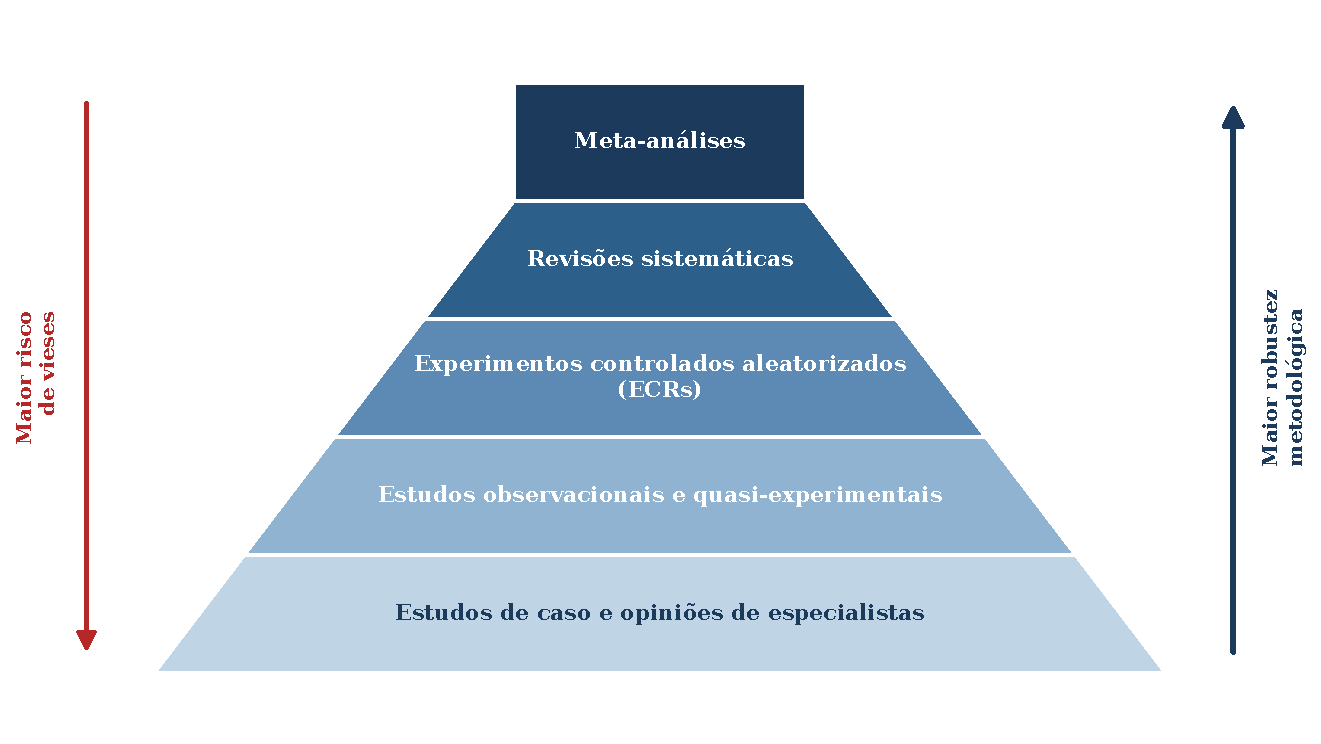
\includegraphics[width=0.85\textwidth]{fig_piramide_evidencias.pdf}
\caption{Pirâmide de evidências: tipos de estudo organizados por nível de
robustez metodológica. Adaptado de \citet{Murad2016}.}
\label{fig:piramide}
\end{figure}

É importante usar essa hierarquia com discernimento. Nem sempre o estudo
metodologicamente mais robusto é o mais relevante para o contexto em questão.
Uma meta-análise produzida com dados de países de alta renda pode ter menos
valor prático para uma política municipal brasileira do que um estudo
qualitativo conduzido em contexto similar.

\section{Por que evidências acadêmicas importam para a gestão pública?}

A gestão pública decide sob incerteza. Raramente há tempo, recursos ou
condições ideais para conduzir uma avaliação completa antes de agir. Nesse
cenário, as evidências acadêmicas funcionam como um atalho qualificado:
permitem aprender com o que outros já fizeram, evitar erros conhecidos e
orientar escolhas com maior base empírica.

Isso não significa que basta consultar a literatura. As evidências precisam
ser combinadas com o conhecimento do contexto local, a experiência técnica e
o conhecimento tácito das equipes, os marcos legais e normativos pertinentes,
a documentação institucional e o julgamento técnico e político. O que as
evidências acadêmicas oferecem é uma camada adicional de rigor e
confiabilidade ao processo decisório.

\begin{notabox}[Pontos-chave]
\begin{itemize}[leftmargin=*]
  \item Comece pelas revisões sistemáticas e meta-análises quando quiser uma
    visão geral sobre o que funciona em determinada área.
  \item Use artigos originais quando precisar aprofundar um contexto
    específico ou compreender os mecanismos de uma intervenção.
  \item Recorra a \textit{policy briefs} quando o tempo for curto ou quando
    precisar comunicar evidências para públicos não técnicos.
  \item Combine as evidências acadêmicas com o conhecimento tácito da equipe,
    os marcos legais e normativos e a documentação institucional disponível.
  \item Nunca baseie uma decisão importante em um único estudo: busque
    corroboração em diferentes fontes.
\end{itemize}
\end{notabox}

% ═══════════════════════════════════════════════════════════════════════════════
% CAPÍTULO 2
% ═══════════════════════════════════════════════════════════════════════════════
\chapter{Onde e como encontrar evidências acadêmicas}\label{cap2}

Saber que as evidências existem é a parte fácil. O difícil vem depois: encontrá-las sem se afogar no volume de publicações e separar o que é relevante para o problema em mãos.

Este capítulo apresenta as principais fontes de evidências acadêmicas para
políticas públicas e oferece orientações práticas para conduzir buscas
produtivas. Uma distinção inicial vale o registro: este guia trata de
\textbf{evidências sistematizadas} --- estudos avaliativos, revisões e
sínteses produzidos pela pesquisa acadêmica. Para o tratamento detalhado de
\textbf{fontes de dados primários e administrativos} (registros públicos,
microdados, sistemas nacionais de informação), recomenda-se a leitura do guia
da série dedicado a fontes de dados para avaliação de políticas públicas.

\section{Principais plataformas e repositórios}

O ecossistema de produção e disseminação de evidências para políticas públicas
cresceu muito nas últimas duas décadas. Gestores e consultores hoje têm
acesso a uma variedade de plataformas que organizam estudos avaliativos,
revisões sistemáticas e sínteses de evidências de forma estruturada e, na
maioria dos casos, gratuita.

\subsection{Plataformas nacionais}

\begin{description}[leftmargin=2em, labelwidth=0pt]
  \item[\textbf{FGV CLEAR} (\url{fgvclear.org})] Centro regional da Global
    Evaluation Initiative para o Brasil e os países lusófonos. Publica guias
    técnicos, estudos avaliativos e materiais de capacitação sobre
    monitoramento e avaliação de políticas públicas.
  \item[\textbf{Impacto IMDS} (\url{impacto.imdsbrasil.org})] Plataforma
    brasileira que reúne estudos avaliativos de políticas sociais com
    linguagem acessível e foco no contexto nacional.
  \item[\textbf{IPEA} (\url{ipea.gov.br})] O Instituto de Pesquisa Econômica
    Aplicada produz e disponibiliza Textos para Discussão, boletins e livros
    com avaliações de políticas públicas brasileiras em diversas áreas
    (sociais, econômicas, urbanas, ambientais).
  \item[\textbf{Fundação João Pinheiro --- FJP}
    (\url{fjp.mg.gov.br})] Centro de pesquisa aplicada vinculado ao governo
    de Minas Gerais, com produção relevante sobre políticas públicas
    estaduais, déficit habitacional, finanças públicas e indicadores
    sociais.
  \item[\textbf{ENAP} (\url{enap.gov.br})] A Escola Nacional de Administração
    Pública publica cadernos, pesquisas aplicadas e materiais sobre gestão
    pública e formulação de políticas.
  \item[\textbf{SciELO Brasil} (\url{scielo.br})] Biblioteca eletrônica que
    reúne periódicos científicos brasileiros em acesso aberto, cobrindo
    diversas áreas. Útil quando o objetivo é encontrar estudos publicados em
    português.
\end{description}

\subsection{Plataformas internacionais}

\begin{description}[leftmargin=2em, labelwidth=0pt]
  \item[\textbf{J-PAL --- Poverty Action Lab} (\url{povertyactionlab.org})]
    Rede global de pesquisadores que realiza e divulga avaliações de impacto
    em países em desenvolvimento, com destaque para experimentos
    aleatorizados.
  \item[\textbf{3ie --- International Initiative for Impact Evaluation}
    (\url{3ieimpact.org})] Produz revisões sistemáticas e mantém um banco de
    dados com centenas de avaliações de impacto em países de baixa e média
    renda.
  \item[\textbf{Campbell Collaboration} (\url{campbellcollaboration.org})]
    Biblioteca internacional de revisões sistemáticas sobre políticas
    sociais, educação, criminologia e bem-estar.
  \item[\textbf{World Bank Open Knowledge Repository}
    (\url{openknowledge.worldbank.org})] Repositório de publicações do Banco
    Mundial que reúne estudos sobre uma variedade de políticas e temas de
    desenvolvimento em diversas regiões do mundo.
  \item[\textbf{What Works Network --- Reino Unido}
    (\url{gov.uk/guidance/what-works-network})] Plataformas governamentais
    com sínteses de evidência sobre setores específicos, como educação,
    saúde e segurança pública.
  \item[\textbf{VoxDev} (\url{voxdev.org})] Publica revisões de literatura
    sobre temas relevantes em desenvolvimento econômico.
  \item[\textbf{Google Scholar} (\url{scholar.google.com})] Motor de busca
    acadêmico de ampla cobertura, útil para identificar artigos e verificar
    citações.
  \item[\textbf{Scopus e Web of Science}] Bases de dados acadêmicas com ampla
    cobertura multidisciplinar, frequentemente acessíveis via universidades
    e instituições de pesquisa.
\end{description}

\subsection{Ferramentas de inteligência artificial para buscas}

Ferramentas de inteligência artificial estão sendo crescentemente utilizadas
para apoiar buscas na literatura acadêmica, e esse cenário evolui com rapidez.
Ferramentas como \textit{Elicit}, \textit{Consensus} e \textit{Research
Rabbit} podem ajudar a identificar estudos relevantes, resumir achados e
mapear redes de citação.

Apesar do potencial, essas ferramentas devem ser usadas com cautela. Resumos
gerados por IA podem conter imprecisões, omitir nuances importantes ou até
mesmo apresentar referências fabricadas (fenômeno conhecido como
``alucinação''). Além disso, a qualidade dos resultados depende da seleção de
fontes feita pela ferramenta, que nem sempre é transparente. O uso adequado
dessas ferramentas pressupõe três cuidados: (i) verificar sempre a existência
e o conteúdo das referências citadas; (ii) ler as fontes originais antes de
incorporá-las a uma análise; e (iii) tratar a IA como ponto de partida para a
descoberta, não como substituto da leitura crítica.

\subsection{Outras formas de busca}

Além das plataformas e repositórios, outras estratégias úteis incluem a busca
manual em periódicos da área de interesse e o rastreamento de citações, que
envolve identificar estudos seminais e analisar tanto suas referências quanto
os trabalhos que os citaram posteriormente. Essas abordagens são mais
trabalhosas, mas essenciais para uma cobertura abrangente do tema.

\section{Como fazer buscas eficientes}

Acessar uma base de dados acadêmica pela primeira vez pode ser desconcertante:
uma busca simples por ``educação'' ou ``saúde pública'' retorna milhares de
resultados, a maioria irrelevante para o problema em questão. Algumas
estratégias ajudam a tornar esse processo mais produtivo, e serão descritas a
seguir. A Figura~\ref{fig:fluxo_busca} resume o fluxo recomendado.

\begin{figure}[h!]
\centering
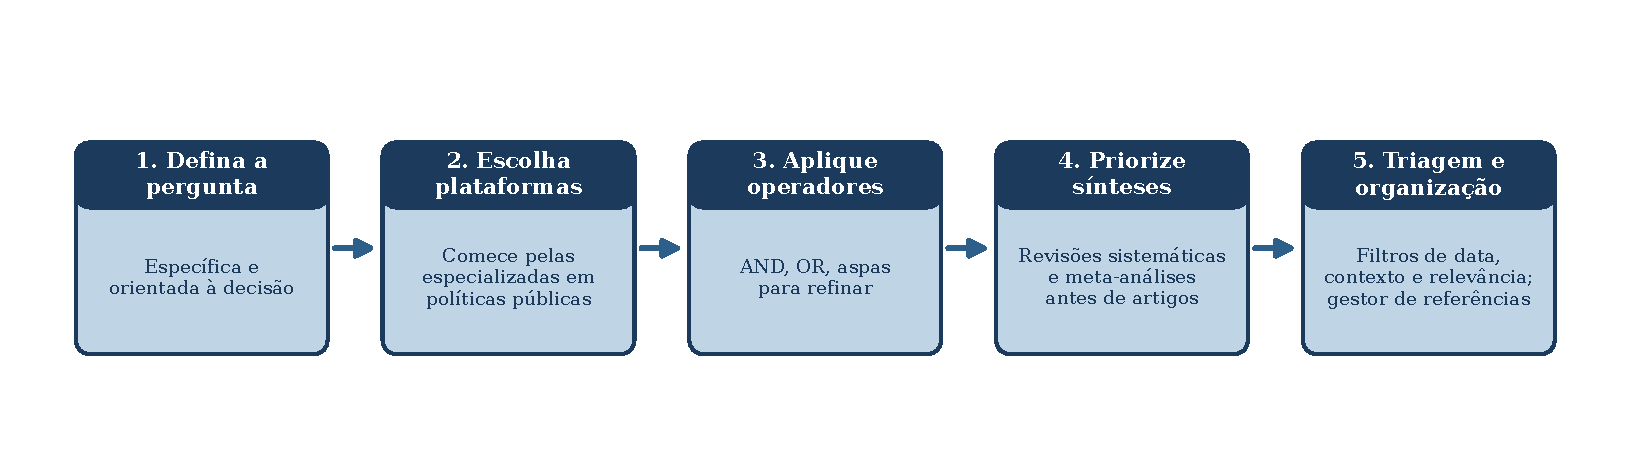
\includegraphics[width=0.95\textwidth]{fig_fluxo_busca.pdf}
\caption{Fluxo recomendado de busca por evidências acadêmicas.}
\label{fig:fluxo_busca}
\end{figure}

\subsection{Defina bem a pergunta antes de buscar}

O erro mais comum cometido na busca por evidências acadêmicas é a utilização
de termos muito vagos. Assim, antes de abrir qualquer plataforma, vale
responder: \textit{qual é exatamente a pergunta que preciso responder?}
Quanto mais específica a pergunta, mais eficiente será a busca. Por exemplo,
em vez de buscar por ``programas sociais para jovens'', uma pergunta mais
precisa seria: ``redução do abandono escolar entre jovens vulneráveis''.

\subsection{Use operadores de busca}

A maioria das plataformas acadêmicas aceita operadores lógicos que refinam os
resultados. Os mais úteis são:

\begin{itemize}[leftmargin=*]
  \item \textbf{AND}: restringe a busca a documentos que contenham todos os
    termos (ex.: \textit{conditional cash transfer AND school attendance});
  \item \textbf{OR}: amplia a busca para documentos que contenham qualquer um
    dos termos (ex.: \textit{dropout OR school abandonment});
  \item \textbf{``aspas''}: busca pela expressão exata
    (ex.: \textit{``early childhood education''}).
\end{itemize}

\subsection{Priorize sínteses antes de artigos individuais}

Quando o objetivo é ter uma visão geral do que a literatura diz sobre um tema,
comece pelas revisões sistemáticas e meta-análises. Elas já fizeram o trabalho
de reunir e avaliar os estudos individuais, poupando tempo e reduzindo o risco
de selecionar estudos que não são representativos do estado do conhecimento.

\subsection{Verifique a data de publicação}

Em áreas de política pública que evoluem rapidamente --- como tecnologia
educacional, saúde mental ou mercado de trabalho ---, estudos com mais de dez
anos podem estar desatualizados. Dê preferência a publicações recentes,
especialmente ao buscar evidências sobre intervenções específicas.

\section{Organizando o material encontrado}

Encontrar os estudos é apenas metade do trabalho. Organizar e sistematizar o
que foi encontrado é igualmente importante, especialmente quando a equipe
precisa compartilhar e usar esse material ao longo do tempo.

Algumas práticas úteis incluem:

\begin{itemize}[leftmargin=*]
  \item Usar ferramentas de gestão de referências como \textit{Zotero}
    (gratuito) ou \textit{Mendeley} para salvar, organizar e citar artigos;
  \item Criar uma tabela-síntese com as principais informações de cada
    estudo: pergunta de pesquisa, contexto, método, principais resultados e
    limitações;
  \item Registrar as buscas realizadas --- quais plataformas, quais termos,
    quais filtros --- para que possam ser reproduzidas ou atualizadas.
\end{itemize}

\begin{notabox}[Pontos-chave]
\begin{itemize}[leftmargin=*]
  \item Comece sempre pelas plataformas especializadas em políticas públicas
    antes de recorrer às bases acadêmicas genéricas.
  \item Defina a pergunta com precisão antes de iniciar a busca.
  \item Prefira revisões sistemáticas e meta-análises quando quiser uma visão
    geral confiável.
  \item Use uma ferramenta de gestão de referências desde o início para não
    perder o rastro do que foi encontrado.
  \item Ferramentas de IA podem ajudar na descoberta, mas sempre leia as
    fontes originais de forma crítica e verifique a existência das
    referências citadas.
\end{itemize}
\end{notabox}

% ═══════════════════════════════════════════════════════════════════════════════
% CAPÍTULO 3
% ═══════════════════════════════════════════════════════════════════════════════
\chapter{Evidências na identificação e diagnóstico do problema}\label{cap3}

Toda política pública começa pela identificação de um problema social que merece atenção do Estado. Definir bem esse problema é uma das tarefas mais exigentes do ciclo --- e uma das mais consequentes. Um diagnóstico mal feito influencia todas as etapas seguintes: a formulação, a implementação e a avaliação. Para um tratamento aprofundado dessa etapa, recomenda-se a leitura do Guia CLEAR de M\&A \citep{Lima2025}.

É aqui que as evidências acadêmicas têm um papel essencial. Elas permitem ir
além das percepções intuitivas, das pressões políticas imediatas e dos dados
administrativos que, embora valiosos, nem sempre capturam a complexidade do
problema.

\section{Para que servem as evidências no diagnóstico?}

Na etapa de identificação e diagnóstico, as evidências acadêmicas cumprem ao menos três funções.

A primeira é \textbf{caracterizar o problema com precisão}. Estudos acadêmicos oferecem dados sobre a magnitude do problema, sua distribuição na população e suas tendências ao longo do tempo. Não apenas confirmam que um problema existe --- ajudam a dimensioná-lo com rigor.

A segunda é \textbf{identificar causas e consequências}. A literatura frequentemente apresenta análises causais que permitem distinguir entre sintomas e raízes de um problema --- distinção que os dados administrativos raramente conseguem fazer sozinhos.

A terceira é \textbf{identificar grupos mais vulneráveis}. Pesquisas com recortes por raça, gênero, território ou faixa etária revelam desigualdades que as médias agregadas escondem, permitindo um diagnóstico mais justo e preciso.

\section{Como usar evidências acadêmicas no diagnóstico}

\subsection{Busque estudos sobre o problema no contexto brasileiro ou em
contextos similares}

O primeiro passo é verificar se há literatura acadêmica sobre o problema que
você está diagnosticando no Brasil ou em países com características
socioeconômicas e institucionais similares. Estudos produzidos em contextos
muito distintos --- como países de alta renda com sistemas de proteção social
consolidados --- podem oferecer \textit{insights} interessantes, mas precisam
ser interpretados com cautela.

\subsection{Use a literatura para construir e validar a árvore do problema}

A árvore do problema é uma ferramenta amplamente usada no diagnóstico de
políticas públicas. Ela organiza visualmente as causas e consequências de um
problema central. As evidências acadêmicas são um insumo valioso para
preencher essa árvore com base empírica --- identificando quais causas têm
mais suporte na literatura e quais relações causais são mais bem documentadas.

\subsection{Combine evidências acadêmicas com dados locais}

Evidências acadêmicas não substituem o conhecimento do contexto local. O ideal
é combiná-las com dados administrativos, registros locais e escutas com a
população afetada. Um estudo nacional sobre evasão escolar, por exemplo, pode
ser complementado com dados municipais para verificar se os padrões descritos
na literatura se reproduzem localmente.

\begin{exemplobox}[Diagnóstico da violência doméstica contra a mulher]
Uma secretaria estadual de segurança pública está elaborando uma política de
enfrentamento à violência doméstica. A equipe técnica parte dos dados de
boletins de ocorrência, mas percebe que esses registros capturam apenas uma
fração dos casos --- a literatura acadêmica indica que a subnotificação pode
chegar a mais de 80\%.

Ao buscar estudos acadêmicos sobre o tema, a equipe identifica pesquisas que
documentam os principais fatores associados à não denúncia: medo de
represálias, dependência econômica, ausência de rede de apoio e desconfiança
nas instituições. Essa informação é fundamental para o diagnóstico, pois
revela que o problema não é apenas a violência em si, mas um conjunto de
condições estruturais que impedem que ele seja identificado e enfrentado.

A equipe também encontra estudos que mostram a maior prevalência do problema
entre mulheres negras, de baixa renda e residentes em áreas periféricas ---
um dado que os boletins de ocorrência, concentrados em regiões com maior
acesso à polícia, não conseguiam revelar. Esse diagnóstico mais preciso
orienta tanto a focalização da política quanto a escolha das intervenções.
\end{exemplobox}

\begin{notabox}[Pontos-chave]
\begin{itemize}[leftmargin=*]
  \item Use a literatura para ir além dos sintomas: utilize referências
    bibliográficas que analisem as causas de um determinado problema
    público, não apenas suas manifestações.
  \item Verifique se as causas identificadas na literatura se confirmam no
    contexto local com dados primários ou administrativos.
  \item Dê atenção especial a estudos com recortes de raça, gênero e
    território --- eles podem revelar desigualdades que os dados agregados
    escondem.
  \item Documente as referências usadas no diagnóstico: isso fortalece a
    legitimidade técnica das escolhas feitas.
\end{itemize}
\end{notabox}

% ═══════════════════════════════════════════════════════════════════════════════
% CAPÍTULO 4
% ═══════════════════════════════════════════════════════════════════════════════
\chapter{Evidências na formulação da política}\label{cap4}

Uma vez que o problema foi bem diagnosticado, começa a etapa de formulação:
definir quais objetivos a política perseguirá, quais intervenções serão
adotadas e como elas se conectam causalmente aos resultados esperados. É nesse
momento que o risco de errar é mais alto --- e também onde as evidências
acadêmicas têm maior potencial de contribuição.

Formular sem consultar o que já foi testado e avaliado é repetir, no escuro, escolhas que outros gestores e pesquisadores já fizeram antes. A literatura acadêmica oferece um repertório de intervenções testadas, com resultados documentados em diferentes contextos. Usá-la bem não significa copiar o que funcionou em outro lugar, mas aprender com essas experiências para desenhar algo mais coerente e mais robusto.

\section{Identificando e comparando alternativas de intervenção}

O primeiro uso das evidências na formulação é ampliar o leque de alternativas
consideradas. Frequentemente, equipes técnicas chegam à fase de formulação com
uma ou duas opções em mente --- geralmente aquelas que já são conhecidas ou
que estão na moda politicamente. A literatura acadêmica permite ir além
dessas opções iniciais, revelando intervenções que funcionaram em contextos
comparáveis e outras que, apesar de intuitivamente atraentes, não produziram
os resultados esperados.

Uma ferramenta útil para organizar essa comparação é a \textbf{matriz de
evidências}, que cruza cada alternativa com informações sobre: contexto em
que foi testada, método de avaliação utilizado, magnitude dos efeitos
encontrados, grupos beneficiados e principais limitações identificadas.

\section{Fundamentando a Teoria da Mudança}

A Teoria da Mudança (TdM) é a representação lógica de como se espera que uma
intervenção produza seus resultados. Ela explicita os insumos mobilizados, as
atividades realizadas, os produtos entregues, os resultados esperados e os
impactos de longo prazo \citep{Lima2025}. Por organizar de forma sistemática a
cadeia causal que conecta a ação da política aos resultados pretendidos, a
TdM é um dos instrumentos centrais da formulação --- e um dos pontos em que a
literatura acadêmica mais contribui. Para um tratamento detalhado da TdM e de
seus componentes, recomenda-se a leitura do Guia CLEAR de M\&A.

As evidências acadêmicas são insumos essenciais para construir uma TdM bem
fundamentada. Elas ajudam a responder: \textit{há evidências de que esse
mecanismo causal realmente funciona?} Por exemplo, se a teoria pressupõe que
oferecer bolsas de estudo a jovens de baixa renda reduz a evasão escolar, a
literatura deve ser consultada para verificar se essa cadeia causal tem
suporte empírico --- e em que condições ela tende a funcionar.

\section{Lidando com lacunas de evidência}

Nem sempre a literatura oferece respostas claras para o contexto em questão.
Pode ser que não haja estudos sobre a intervenção considerada no Brasil, ou
que os estudos disponíveis sejam metodologicamente frágeis. Nessas situações,
algumas estratégias são úteis:

\begin{itemize}[leftmargin=*]
  \item Buscar evidências em contextos análogos --- países com estrutura
    institucional, nível de renda ou características culturais similares;
  \item Recorrer a modelos teóricos que expliquem os mecanismos pelos quais a
    intervenção deve funcionar, mesmo na ausência de avaliações diretas;
  \item Planejar a política com um componente de avaliação de impacto ou de
    resultados embutida desde o início, de modo a gerar evidências sobre
    essa intervenção específica que ainda não existem na literatura
    \citep{Imas2009}.
\end{itemize}

\begin{exemplobox}[Formulação de um programa de habitação social]
Um estado está desenhando um programa de habitação para famílias em situação
de vulnerabilidade. A equipe considera duas alternativas principais:
construção de conjuntos habitacionais em áreas periféricas ou concessão de
subsídios para aluguel em localidades escolhidas pelas famílias.

A busca na literatura revela um conjunto robusto de estudos que avaliam
programas de \textit{voucher} habitacional nos Estados Unidos --- especialmente
o programa \textit{Moving to Opportunity} --- e mostram que famílias que se
mudaram para bairros de menor vulnerabilidade apresentaram melhoras
significativas em saúde mental, desempenho escolar dos filhos e renda de
longo prazo \citep{Chetty2016}. Ao mesmo tempo, estudos brasileiros e
latino-americanos indicam que conjuntos habitacionais em áreas periféricas
frequentemente reproduzem condições de isolamento social e acesso precário a
equipamentos e serviços urbanos \citep{Cardoso2013}.

Com base nessa revisão, a equipe decide avançar com o modelo de subsídio ao
aluguel, incorporando à Teoria da Mudança as condições que a literatura
aponta como necessárias para o sucesso da intervenção: acompanhamento social
das famílias, articulação com políticas de emprego e acesso a transporte
público.
\end{exemplobox}

\begin{notabox}[Pontos-chave]
\begin{itemize}[leftmargin=*]
  \item Antes de formular, pesquise o que já foi testado: evite reinventar
    intervenções cujos resultados já são conhecidos.
  \item Use a literatura para verificar se a cadeia causal da sua Teoria da
    Mudança tem suporte empírico.
  \item Quando houver lacunas de evidência, busque contextos análogos e
    documente as incertezas e premissas assumidas.
  \item Planeje a avaliação da política desde a formulação, especialmente
    quando as evidências disponíveis forem escassas.
\end{itemize}
\end{notabox}

% ═══════════════════════════════════════════════════════════════════════════════
% CAPÍTULO 5
% ═══════════════════════════════════════════════════════════════════════════════
\chapter{Evidências na implementação}\label{cap5}

Mesmo uma política bem formulada pode falhar na implementação. As evidências
acadêmicas têm um papel importante nessa etapa, embora menos óbvio do que
nas fases de diagnóstico e formulação. Elas ajudam a antecipar riscos,
informar o monitoramento e orientar correções de rota durante a execução.

\section{Antecipando riscos com base na literatura}

Antes mesmo de a política entrar em operação, a literatura acadêmica pode ser
consultada para identificar os principais desafios de implementação de
intervenções semelhantes. Esses desafios raramente são exclusivos de um
contexto --- ao contrário, muitos se repetem de forma reconhecível em
diferentes países e setores.

Alguns exemplos de perguntas que a literatura pode ajudar a responder nessa
etapa:

\begin{itemize}[leftmargin=*]
  \item Quais são as barreiras típicas de adesão do público-alvo a este tipo
    de intervenção?
  \item Quais capacidades institucionais são necessárias para executar esse
    tipo de política com qualidade?
  \item Quais foram os principais problemas operacionais relatados em
    experiências similares?
\end{itemize}

\section{Informando o plano de monitoramento}

O plano de monitoramento define quais indicadores serão acompanhados durante
a implementação, com qual periodicidade e por quem \citep{Lima2025}. A
literatura acadêmica pode contribuir para esse plano ao indicar quais
variáveis se mostraram mais sensíveis à qualidade da implementação em
intervenções semelhantes --- ou seja, quais sinais de alerta devem ser
observados com mais atenção.

Além disso, estudos sobre avaliação de processos oferecem \textit{frameworks}
úteis para estruturar o monitoramento. Para acompanhar uma implementação com
profundidade, é importante ir além dos indicadores de cobertura e considerar
um conjunto de \textbf{dimensões da qualidade da implementação}, entre as
quais se destacam: (i) a \textit{fidelidade} ao desenho --- a intervenção
está sendo entregue como planejada?; (ii) a \textit{dose ou intensidade}
recebida pelos beneficiários; (iii) o \textit{alcance} efetivo do
público-alvo; (iv) a \textit{qualidade da entrega} --- competência das
equipes, condições de infraestrutura, padronização dos protocolos; e (v) a
\textit{responsividade} dos beneficiários --- nível de engajamento e
participação efetiva. A literatura sobre intervenções similares ajuda a
identificar quais dessas dimensões merecem mais atenção em cada caso.

\section{Orientando correções de rota}

Durante a implementação, é comum que problemas não previstos apareçam.
Quando isso acontece, a equipe gestora precisa decidir rapidamente se deve
ajustar a intervenção ou mantê-la como planejado. A literatura acadêmica pode
informar essa decisão, especialmente quando o problema identificado já foi
descrito e analisado em outros contextos.

\begin{exemplobox}[Implementação de um programa de visitas domiciliares para
gestantes]
Um estado implementa um programa de visitas domiciliares de agentes
comunitários de saúde a gestantes de alto risco. Nos primeiros meses de
operação, o monitoramento revela baixas taxas de adesão: muitas gestantes
recusam as visitas ou não estão em casa nos horários agendados.

A equipe busca na literatura estudos sobre a implementação de programas
similares e encontra pesquisas que identificam barreiras recorrentes:
desconfiança inicial das famílias, horários incompatíveis com a rotina das
beneficiárias e percepção de que as visitas têm caráter fiscalizatório em
vez de apoio. Os estudos também documentam estratégias que mostraram ser
eficazes para superar essas barreiras: envolvimento das lideranças
comunitárias no recrutamento, flexibilização dos horários e clareza na
comunicação sobre os objetivos do programa.

Com base nessas evidências, a equipe realiza ajustes operacionais sem
precisar reformular toda a política --- uma correção de rota fundamentada,
que aumenta a probabilidade de o programa alcançar os resultados esperados.
\end{exemplobox}

\begin{notabox}[Pontos-chave]
\begin{itemize}[leftmargin=*]
  \item Consulte a literatura sobre implementação de programas similares
    \emph{antes} do lançamento: muitos problemas operacionais são
    previsíveis.
  \item Use as evidências para definir quais indicadores de processo merecem
    mais atenção no monitoramento.
  \item Quando surgirem problemas na implementação, verifique se a literatura
    já documentou esse tipo de falha e como outros a superaram.
  \item Distingua falhas de implementação de falhas de teoria: a literatura
    pode ajudar a fazer esse diagnóstico com mais precisão.
\end{itemize}
\end{notabox}

% ═══════════════════════════════════════════════════════════════════════════════
% CAPÍTULO 6
% ═══════════════════════════════════════════════════════════════════════════════
\chapter{Evidências na análise de resultados e impactos}\label{cap6}

Implementada a política, chega o momento de entender seus efeitos: o que mudou? Para quem? Em que magnitude? A que custo? São as perguntas que organizam a avaliação de resultados e impactos --- e nesta etapa as evidências acadêmicas cumprem um papel que vai além da metodologia.

Para além de orientar o desenho da avaliação, a literatura serve como \textbf{referência comparativa}: contextualiza os resultados encontrados, ajuda a verificar se os efeitos observados são consistentes com o que se esperaria à luz do conhecimento existente e indica o que pode explicar eventuais discrepâncias.

\section{A literatura como referência comparativa (\textit{benchmark})}

Um dos usos mais valiosos --- e menos explorados --- das evidências acadêmicas
na fase de análise é a comparação dos resultados obtidos com os efeitos
documentados em intervenções similares. Essa comparação permite responder a
perguntas como:

\begin{itemize}[leftmargin=*]
  \item O efeito encontrado é compatível com o que a literatura reporta para
    esse tipo de intervenção?
  \item O tamanho do efeito está acima ou abaixo da média observada em
    contextos similares?
  \item Se os resultados foram mais limitados do que o esperado, o que a
    literatura sugere como possíveis explicações?
\end{itemize}

\section{Interpretando resultados inesperados}

Não raro, avaliações de políticas públicas produzem resultados surpreendentes:
efeitos menores do que o esperado, ausência de impacto ou até efeitos
negativos --- ou seja, intervenções que agravam o problema em vez de
remediá-lo. Nesses casos, a literatura acadêmica pode ajudar a formular
hipóteses explicativas.

Duas categorias de explicação são especialmente relevantes e podem ser
iluminadas pela pesquisa acadêmica \citep{Lima2025}:

\begin{description}[leftmargin=2em]
  \item[\textbf{Falha de implementação}] A intervenção não foi executada como
    planejada --- houve baixa cobertura, qualidade insuficiente da entrega,
    rotatividade alta de equipes, atrasos sistemáticos no fluxo operacional
    ou outros problemas de execução. Estudos sobre implementação de
    programas similares podem indicar se esses problemas são recorrentes
    nesse tipo de intervenção.
  \item[\textbf{Falha de teoria}] Ainda que implementada conforme o
    planejado, a lógica causal por trás da política se mostra frágil ou não
    considera fatores determinantes para o problema que se pretende
    enfrentar --- a execução ocorre como previsto, mas não produz os
    resultados almejados. Por exemplo, um programa de capacitação
    profissional pode ser executado com excelência operacional e ainda
    assim não melhorar a empregabilidade dos beneficiários, se o problema
    central não for a qualificação, mas a escassez de vagas no mercado
    local. A literatura teórica e empírica sobre o problema pode ajudar a
    identificar se essa é a explicação mais plausível.
\end{description}

\section{Comunicando resultados com base na literatura}

Ao apresentar os resultados de uma avaliação para gestores, formuladores ou a
sociedade, contextualizar os achados com referências à literatura acadêmica
fortalece a credibilidade da análise, facilita a interpretação e pode nortear
eventuais correções necessárias para que a política atinja seus objetivos.
Em vez de apresentar um número isolado, o avaliador pode situá-lo em relação
ao que se sabe sobre intervenções similares --- tornando os resultados mais
compreensíveis e as recomendações mais bem fundamentadas.

\begin{exemplobox}[Avaliação de um programa de transferência de renda para
jovens em vulnerabilidade]
Um estado avalia um programa de transferência de renda condicional voltado a
jovens de 16 a 24 anos em situação de vulnerabilidade, com condicionalidades
vinculadas à frequência escolar e à participação em cursos de qualificação
profissional. Após dois anos, a avaliação identifica uma redução de 12 pontos
percentuais na taxa de abandono escolar entre os beneficiários.

A equipe de avaliação consulta a literatura para contextualizar esse
resultado. Revisões sistemáticas sobre programas de transferência de renda
condicional em países de baixa e média renda reportam efeitos médios sobre
frequência escolar entre 5 e 15 pontos percentuais, dependendo do desenho do
programa e do contexto \citep{Baird2014}. O resultado encontrado está,
portanto, dentro do intervalo esperado --- o que reforça a plausibilidade da
estimativa.

Ao mesmo tempo, a avaliação não encontra efeitos significativos sobre
empregabilidade após o encerramento do programa. A literatura sugere que
intervenções de curta duração raramente produzem mudanças sustentadas no
mercado de trabalho sem componentes de inserção produtiva mais estruturados
\citep{Kluve2016}. Esse achado orienta uma recomendação específica: ampliar
o componente de intermediação de emprego da política para o próximo ciclo.
\end{exemplobox}

\begin{notabox}[Pontos-chave]
\begin{itemize}[leftmargin=*]
  \item Use a literatura para criar uma referência comparativa: qual é o
    efeito típico desse tipo de intervenção?
  \item Resultados abaixo do esperado podem indicar falha de implementação ou
    falha de teoria --- a literatura ajuda a distinguir.
  \item Resultados acima do esperado também merecem verificação: podem
    refletir um contexto favorável ou problemas metodológicos na avaliação.
  \item Ao comunicar resultados, situe os achados em relação ao que a
    literatura reporta: isso aumenta a credibilidade e facilita a
    interpretação.
\end{itemize}
\end{notabox}

% ═══════════════════════════════════════════════════════════════════════════════
% CAPÍTULO 7
% ═══════════════════════════════════════════════════════════════════════════════
\chapter{Limites e armadilhas no uso de evidências acadêmicas}\label{cap7}

Os capítulos anteriores defendem que as evidências acadêmicas são insumo valioso em todas as etapas do ciclo da política pública. Mas seria ingênuo concluir que mais evidências sempre levam a melhores políticas --- o uso acrítico, seletivo ou descontextualizado da literatura pode ser tão problemático quanto ignorá-la.

Este capítulo apresenta os principais limites e armadilhas no uso de
evidências acadêmicas --- não para desestimular seu uso, mas para promover
uma postura mais crítica, reflexiva e responsável.

\section{Transferência acrítica de resultados entre contextos}

Uma das armadilhas mais comuns é assumir que o que funcionou em um contexto
funcionará da mesma forma em outro. A literatura acadêmica está repleta de
avaliações de intervenções realizadas em países de alta renda, com contextos
institucionais, culturais e econômicos muito distintos da realidade
brasileira. Transportar esses resultados sem análise crítica pode levar a
escolhas inadequadas.

Antes de usar um estudo como referência para uma decisão de política, vale
perguntar: em que contexto foi conduzido? Quais características do contexto
podem ser relevantes para os resultados? Há evidências de que o mecanismo
causal opera de forma semelhante no Brasil?

\section{Uso seletivo de evidências}

Outro risco frequente é o chamado \textit{cherry-picking}: selecionar apenas
os estudos que confirmam a decisão que já havia sido tomada, ignorando a
literatura que aponta em direção contrária. Esse comportamento, muitas vezes
não intencional, compromete a integridade do processo decisório e pode levar
a políticas mal fundamentadas.

Uma forma de mitigar esse risco é adotar uma abordagem sistemática na
revisão da literatura --- documentando os critérios de inclusão e exclusão
dos estudos consultados e registrando tanto as evidências favoráveis quanto
as desfavoráveis à intervenção considerada.

\section{Excesso de confiança em um único estudo}

Um estudo com metodologia rigorosa e resultados expressivos pode ser muito
persuasivo. Mas um único estudo, por mais bem conduzido que seja, raramente
é suficiente para fundamentar uma decisão de política. Os resultados podem
não se replicar em outros contextos, o estudo pode ter limitações não
explicitadas, ou pode ser um achado atípico em relação ao conjunto da
literatura.

A regra geral é buscar corroboração: verifique se os resultados encontrados
em um estudo são consistentes com o que reportam outros estudos sobre
intervenções similares.

\section{A ilusão da evidência como substituto do julgamento}

Por fim, vale resistir à tentação de tratar as evidências acadêmicas como
oráculo que dispensa o julgamento técnico e político. As evidências informam,
mas não decidem. Reduzem a incerteza, mas não a eliminam. E, com frequência,
a literatura não oferece resposta direta para o problema específico --- exige
interpretação, adaptação e ponderação.

O trabalho do gestor não é achar \textit{a} evidência que diz o que fazer ---
é articular múltiplas fontes (incluindo as acadêmicas) para construir o
melhor julgamento possível sobre como agir.

\begin{atencaobox}[Cuidados essenciais]
\begin{itemize}[leftmargin=*]
  \item Verifique sempre o contexto em que um estudo foi conduzido antes de
    usá-lo como referência para uma decisão de política.
  \item Avalie a confiabilidade metodológica do estudo: amostra, desenho de
    identificação causal e revisão por pares são pistas importantes.
  \item Documente tanto as evidências favoráveis quanto as desfavoráveis à
    intervenção considerada.
  \item Nunca baseie uma decisão importante em um único estudo: busque
    corroboração.
  \item Verifique possíveis conflitos de interesse na produção da pesquisa
    consultada.
  \item Lembre-se: evidências informam o julgamento, mas não o substituem.
\end{itemize}
\end{atencaobox}

% ═══════════════════════════════════════════════════════════════════════════════
% REFERÊNCIAS
% ═══════════════════════════════════════════════════════════════════════════════
\bibliographystyle{plainnat}
\bibliography{referencias}

\end{document}